\documentclass[10pt,twoside]{article}
\usepackage[utf8]{inputenc}
\usepackage{amsmath}
\usepackage{amsfonts}
\usepackage{amssymb}
\usepackage[spanish,es-noshorthands]{babel}
\usepackage[T1]{fontenc}
\usepackage{lmodern}
\usepackage{graphicx,hyperref}
\usepackage{tikz,pgf}
\usepackage{multicol}
\usepackage{subfig}
\usepackage[papersize={6.5in,8.5in},width=5.5in,height=7in]{geometry}
\usepackage{fancyhdr}
\pagestyle{fancy}
\fancyhead[LE]{
\includegraphics[height=12pt]{Images/logo-colegio.png} Estadística $6^{\circ}$}
\fancyhead[RE]{}
\fancyhead[RO]{\textit{Germ\'an Avenda\~no Ram\'irez, Lic. U.D., M.Sc. U.N.}}
\fancyhead[LO]{}

\author{Germ\'an Avenda\~no Ram\'irez, Lic. U.D., M.Sc. U.N.}
\title{\begin{minipage}{.2\textwidth}

\includegraphics[height=1.75cm]{Images/logo-colegio.png}\end{minipage}
\begin{minipage}{.55\textwidth}
\begin{center}
Taller 02, Gráficas  \\
Estadística $6^{\circ}$
\end{center}
\end{minipage}\hfill
\begin{minipage}{.2\textwidth}

\includegraphics[height=1.75cm]{Images/logo-sed.png} 
\end{minipage}}
\date{}
\begin{document}
\maketitle
Nombre: \hrulefill Curso: \underline{\hspace*{44pt}} Fecha: \underline{\hspace*{2.5cm}}
\section*{Gr\'afica lineal (1)}
Un grupo de estudiantes registra la temperatura que hay a las 12:00 del mediodía durante 10 días. Presenta sus resultados en un gráfica lineal. Observe:
\begin{center}
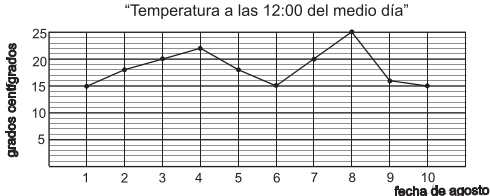
\includegraphics[scale=.75]{Images/grafica1.png} 
\end{center}
\begin{enumerate}
\item Observe la gráfica y responda:
\begin{enumerate}
\item ¿Qué información encuentra en el eje vertical?
\item ¿Qué información encuentra en el eje horizontal?
\item ¿Cuántos grados centígrados indica cada gradación del eje vertical?
\item ¿Qué temperatura hubo el 4 de agosto?
\item ¿En qué fechas se dio una temperatura de 18 grados centígrados?
\item ¿Qué fechas se dio la temperatura más alta?
\item ¿Qué fechas se dio la temperatura más baja?
\item ¿Cuántos grados subió la temperatura entre el 1 y el 4 de agosto?
\item ¿Este registro se realizaría en un lugra frío o cálido? ¿Por qué piensa eso?
\end{enumerate}
Una persona registra los cambios de temperaturas durante 8 horas
\item Observe la gr\'{a}fica y responda

\begin{minipage}{.4\textwidth}
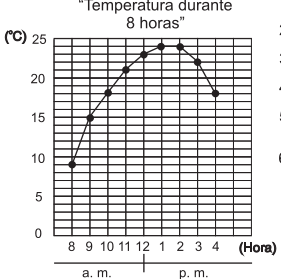
\includegraphics[scale=.6]{Images/grafica2.png} 
\end{minipage}
\begin{minipage}{.55\textwidth}
\begin{enumerate}
\item ¿Qué representa el eje vertical?
\item ¿Qué representa el eje horizontal?
\item ¿Cuánto midió la temperatura a las 10:00?
\item ¿A qué hora la temperatura fue de 15 grados?
\item ¿Cuál fue la temperatura más alta? ¿En cuales horas ocurrió?
\item ¿A qué hora ocurrió la temperatura más baja?
\end{enumerate}
\end{minipage}
\end{enumerate}
\section*{Gráfica lineal (2)}
Lea, observe y aprenda

En la gráfica lineal se puede entender un cambio por la inclinación de la línea, más grande es el cambio
\begin{center}
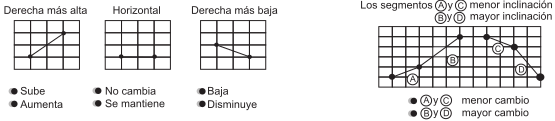
\includegraphics[scale=.65]{Images/graficalineal03.png} 
\end{center}
\begin{enumerate}
\item Observa esta gráfica y responda.
\begin{center}
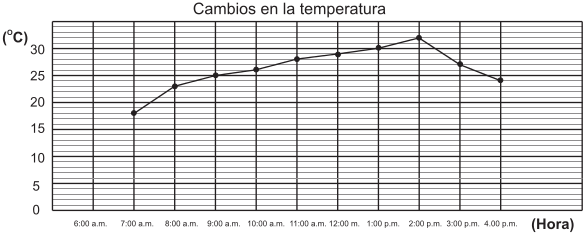
\includegraphics[scale=.65]{Images/grafica04.png} 
\end{center}
\begin{enumerate}
\item A partir de las 7:00 a.m. ¿hasta qué hora dejó de subir la temperatura?
\item ¿A partir de qué hora y hasta qué hora bajó la temperatura?
\item ¿A partir de qué hora y hasta qué hora fue que más bajó la temperatura?
\item ¿Cómo cree que será la temperatura después de las 4:00 p.m.?
\end{enumerate}
\item Observe la gráfica y responda:

\begin{minipage}{.5\textwidth}
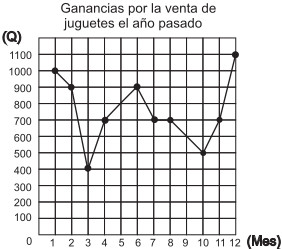
\includegraphics[scale=.75]{Images/grafica05.png} 
\end{minipage}
\begin{minipage}{.5\textwidth}
\begin{enumerate}
\item ¿Cuántos quetzales representa cada gradación del eje vertical?
\item ¿En qué mes hubo más ganancia?
\item ¿Cuántos quetzales se ganaron en abril?
\item ¿En qué mes se ganaron 500 quetzales?
\item ¿A partir de qué mes y hasta qué mes aumentó la ganancia?
\item ¿Cuando no hubo cambio de ganancia?
\item ¿A partir de qué mes y hasta qué mes fue que más aumentó la ganancia?
\item A partir de qué mes y hasta qué mes fue que más disminuyó la ganancia?
\end{enumerate}
\end{minipage}
\end{enumerate}
\section*{Gr\'{a}fica lineal (3)}
\begin{enumerate}
\item Observe las gr\'{a}ficas. Compare y responda.

Un doctor toma la temperatura de un niño. Despu\'{e}s elabora dos gr\'{a}ficas. Observe:
\begin{center}
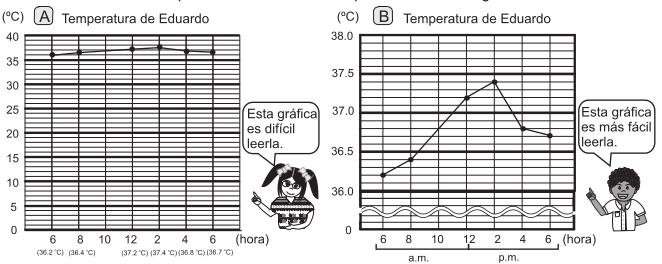
\includegraphics[scale=.52]{Images/grafica06.png} 
\end{center}
\begin{enumerate}
\item ¿Cuáles son las diferencias entre las dos gráficas?
\item ¿En cuál de las dos gráficas es más fácil leer el cambio? ¿Por qué?
\end{enumerate}
\fbox{\begin{minipage}{.95\textwidth}En la gráfica lineal se puede omitir parte de la gradación con el símbolo $\approx$. También se puede cambiar los valores de las gradaciones. Esto se hace para representar los datos de manera más comprensible\end{minipage}}
\item Observe las gráficas anteriores y responda

\begin{minipage}{.65\textwidth}
\begin{enumerate}
\item ¿Bajará o subirá la temperatura del niño a las 10:00 a.m.?
\item Si la temperatura sigue cambiando del mismo modo que a partir de las 4:00 p.m. hasta las 6:00 p.m., ¿cuántos grados centígrados tendrá a las 8:00 p.m.?
\end{enumerate}
\end{minipage}
\begin{minipage}{.35\textwidth}
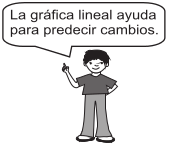
\includegraphics[scale=.55]{Images/nino.png} 
\end{minipage}
\item Observe la gráfica y responda.

\begin{minipage}{.4\textwidth}
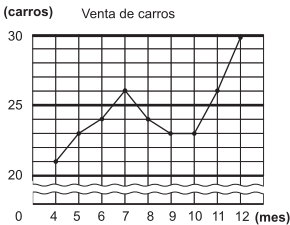
\includegraphics[scale=.6]{Images/grafica07.png} 
\end{minipage}
\begin{minipage}{.55\textwidth}
\begin{enumerate}
\item ¿Qu\'{e} representa el eje vertical?
\item ¿Qu\'{e} representa el eje horizontal?
\item ¿Cu\'{a}ntos carros representa el valor m\'{i}nimo de las gradaciones del eje vertical?
\item ¿Entre qu\'{e} meses fue que m\'{a}s aument\'{o} la venta de carro?
\item ¿Cu\'{a}ntos carros se vendieron en diciembre?
\item ¿Entre qu\'{e} meses fue que baj\'{o} la venta de carros?
\end{enumerate}
\end{minipage}
\end{enumerate}
\end{document}
